%----------------------------------------------------------------------------------------
%	PACKAGES AND OTHER DOCUMENT CONFIGURATIONS
%----------------------------------------------------------------------------------------
\documentclass[12pt]{article}											% font size

\usepackage{amssymb}
\usepackage{amsmath,amsfonts}
\usepackage{subfig}
\usepackage{graphicx}													% to include images
\usepackage{float}														% to float figures
\usepackage{booktabs,makecell}											% for diagonal cells
\usepackage{hyperref}													% for hyperlinks
\usepackage{listings}													% for including files
\usepackage[top=1in, bottom=1in, left=1.25in, right=1.25in]{geometry}	% set margins
\usepackage[utf8]{inputenc}												% for unicode input characters
\usepackage{helvet}														% use helvetica per default
\usepackage{hyperref}													% for hyperlinks
\usepackage[T1]{fontenc}
\usepackage[english]{babel}
\usepackage{color}

\renewcommand{\familydefault}{\sfdefault}								% use sans serif per default

\definecolor{codegreen}{rgb}{0,0.6,0}									%New colors defined below
\definecolor{codegray}{rgb}{0.5,0.5,0.5}
\definecolor{codepurple}{rgb}{0.58,0,0.82}
\definecolor{backcolour}{rgb}{0.95,0.95,0.92}

\lstdefinestyle{mystyle}{												%Code listing style named "mystyle"
  backgroundcolor=\color{backcolour},   commentstyle=\color{codegreen},
  keywordstyle=\color{magenta},
  numberstyle=\tiny\color{codegray},
  stringstyle=\color{codepurple},
  basicstyle=\footnotesize,
  breakatwhitespace=false,         
  breaklines=true,                 
  captionpos=b,                    
  keepspaces=true,                 
  numbers=left,                    
  numbersep=5pt,                  
  showspaces=false,                
  showstringspaces=false,
  showtabs=false,                  
  tabsize=2
}

\lstset{style=mystyle}													%"mystyle" code listing set

% ----------------------------------------------------------------------------------------
%	TITLE SECTION 
% ----------------------------------------------------------------------------------------

\makeatletter
\makeatother
\renewcommand{\familydefault}{\sfdefault}								% use sans serif per default
\makeatother
\title
{
	Machine learning\\
    \emph{Compare different supervised learning algorithms}
}
\author{Riyane SID-LAKHDAR}
\date{\today}


\begin{document}
\maketitle

\begin{abstract}
This document presents the study that we have leaded in order to compare 3 supervised-learning algorithms, namely \emph{Perceptron}, \emph{Logistic Regression}, \emph{AdaBoost}.\\
We present the results that we have obtained in term of learning and testing error, as well as the way they have peen processed.   We also show the scope and the limit of such a benchmark.
\end{abstract}
\tableofcontents
\newpage



%------------------------------
\section{Compare the accuracy of the learning algorithms}
In order to compare the accuracy of the considered learning algorithm, we have first built different set of samples.   Each sample set is split into a learning and a testing set \footnote{Randomly split with a uniform probability distribution of .6 to be in the learning set}.    Then we have run each learning algorithm on each training set.   The Figure \ref{learningAlgoComparison.png} shows for each leaning algorithm the learning and testing error:
\begin{itemize}
	\item The bar charts represent the mean error over all the test sets
	\item The error bar top represents the maximum value of the error over all the test sets
	\item The error bar bottom represents the minimum value of the error over all the test sets
\end{itemize}



\begin{figure*}[t]
\begin{center}
	\subfloat[Row data]
    {
		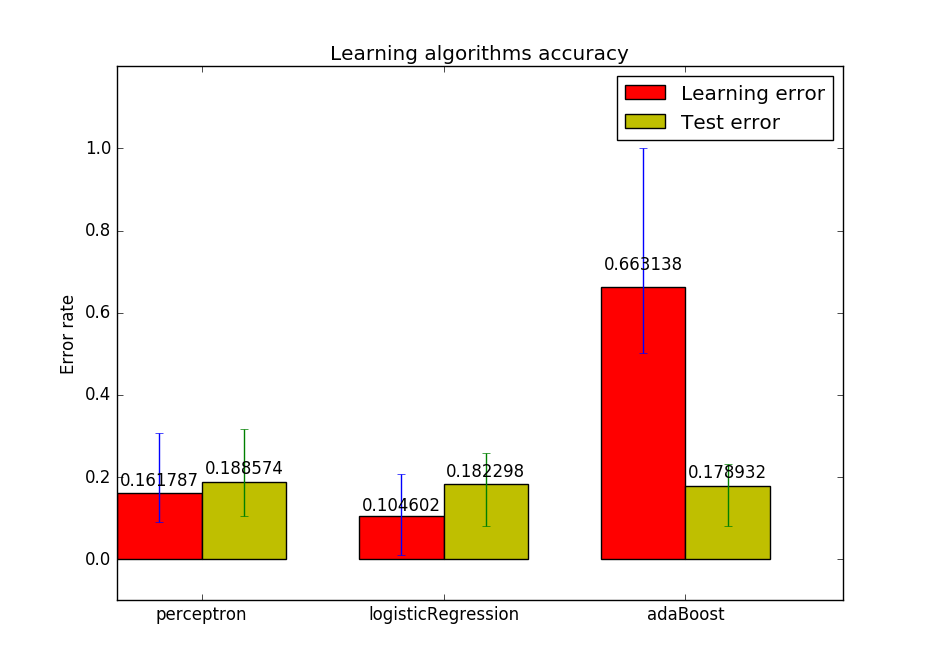
\includegraphics[width=.6\hsize]{chart/learningAlgoComparison.png}
	}
	\subfloat[Normalized data]
    {
		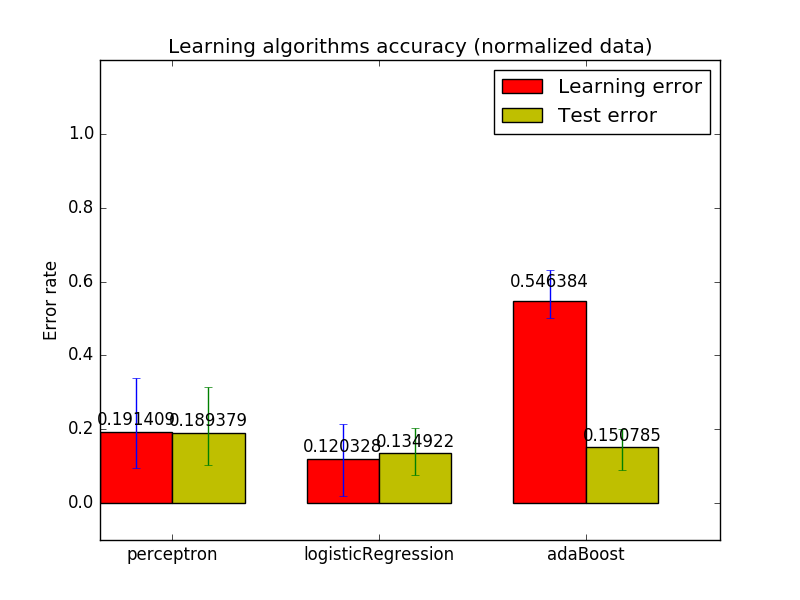
\includegraphics[width=.6\hsize]{chart/learningAlgoComparison_normalized.png}
	}
	\caption{Compare the accuracy of 3 supervised-learning algorithms: \emph{Perceptron}, \emph{Logistic Regression}, \emph{AdaBoost}.}
	\label{learningAlgoComparison.png}
\end{center}
\end{figure*}


Thanks to the Figure  \ref{learningAlgoComparison.png}, one can first notice that the \emph{Logistic Regression} learning algorithm is the most accurate considered algorithm on the considered data sets.   Indeed and mainly when we consider the normalized data, the \emph{Logistic Regression} algorithm has the lowest learning and test error considering the average, minimum and maximum errors.\\

Another noteworthy point on the Figure \ref{learningAlgoComparison.png} is that the \emph{AdaBoost} algorithm does not improve the test error of the \emph{Perceptron} and the \emph{Logistic Regression} algorithms, however it has been proven to be a \emph{boosting} algorithm \footnote{Create a \emph{"strong"} classifier by combining the \emph{"weak"} classifiers \emph{Perceptron} and Logistic Regression }(see previous homework) and that it combines them.\\
One of the possible reasons for this performance drawback is the number of iterations performed by the \emph{AdaBoost} and the two other algorithms:\\
We know for instance that if there exist an optimal parameter (minimizes the learning error), then the \emph{Perceptron} algorithm will converge to in at most $\frac{R}{\rho} ^2$ steps \footnote{Novikoff, 1962, where R is the maximum training vector size and $\rho$ the minimum labeled scalar product of a training vector and the unitary optimal parameter}.   But in most considered training sets, R is smaller than 1 (mainly for the normalized data sets).   Thus this threshold iteration number will be relatively small.
Meanwhile, we have proved (see previous homework) that the empirical error of the \emph{AdaBoost} algorithm decreases exponentially with the number of iterations (number of weak classifiers) \footnote{given that each classifier is slightly better than a coin toast}, the number of weak classifiers used in our implementation (3 weak classifiers) is not sufficient regarding the number of iterations that is performed (maximum 10 iterations).


%------------------------------
\section{Confidence in the obtained results}
In order to assess the confidence in the previously presented results, we have computed the standard deviation of the error of each learning algorithm (after 7 consecutive runs on all the considered data set).   The results are presented on Figure \ref{learningAlgoComparison_stdDeviation.png}.

\begin{figure*}[t]
\begin{center}
	\subfloat
    {
		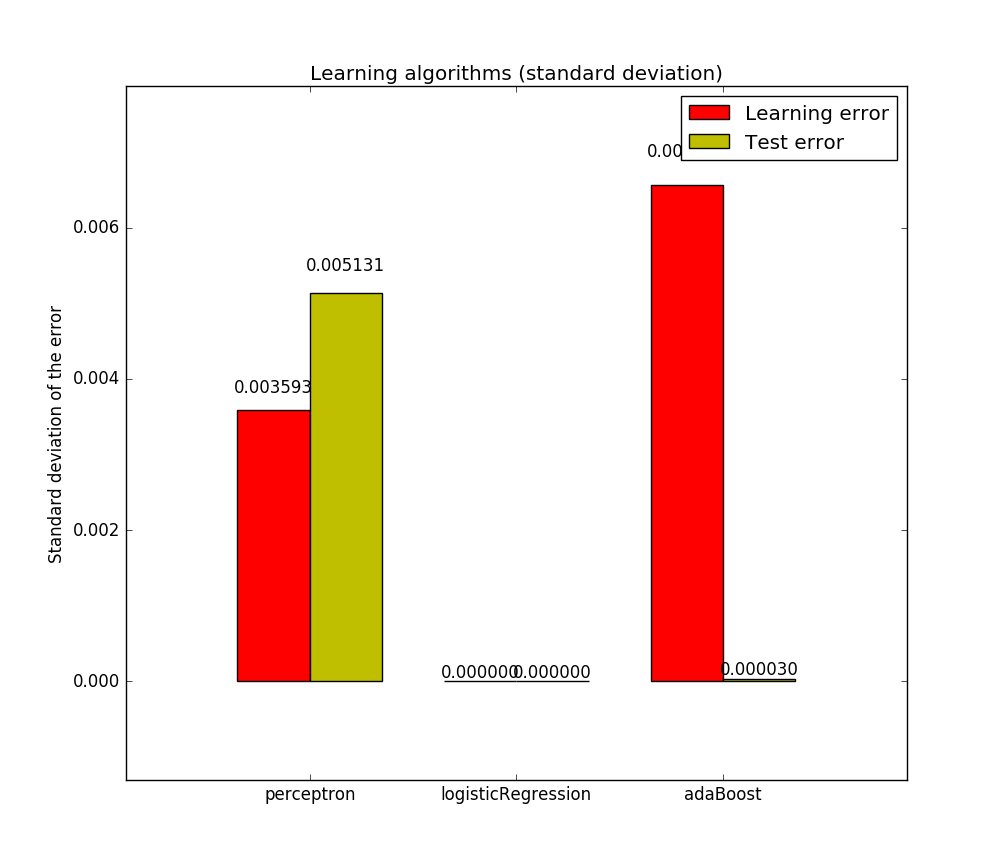
\includegraphics[width=.6\hsize]{chart/learningAlgoComparison_errorStandardDeviation.png}
	}
	\caption{Standard deviation of the learning algorithm error after 7 run on each considered data set.}
	\label{learningAlgoComparison_stdDeviation.png}
\end{center}
\end{figure*}


First, we can notice that standard deviation of the error of all the considered algorithms is smaller than $6 * 10^{-3}$.   Thus, the previously computed error are pretty constant on all the considered data sets and for different iterations.   Hence, the previous results have an interesting confidence property.\\

Second, we can notice that the standard deviation of the \emph{Logistic Regression} algorithm is close to zero (smaller than the considered granularity).   Thus, this algorithm is once again the most accurate one in terms of constancy.


%------------------------------
\section{Experiences} \label{section_experiences}
All the materials that have been used to produce the previously presented experiences may be found at the following address:\\
\href{https://github.com/simbadSid/machineLearning_supervisedLearningComparison.git}{https://github.com/simbadSid/machineLearning\_supervisedLearningComparison.git}\\
The noteworthy directories of this project are the following:
\begin{itemize}
	\item \emph{resource:}   Contains all the row data that are used for the training and the test steps.   It also contains the data generated by our implementation using this row data (normalized data, swap data between training and test sets)


	\item \emph{src:}   Contains all the source code that has been used for the experience.   A unique "Makefile" has been implemented at the root of the directory.   Our code has been separated as follows:
    \begin{itemize}
		\item \emph{learningAlgo:} contains an implementation of each considered algorithm.   Each implementation has been modified (compared to the one given \href{http://ama.liglab.fr/~amini/DataCode.html}{\textbf{at this link}}) in order to communicate with the implemented result printer(see next point).   We have also uniformed the outputs and corrected some bugs noticed in the original codes (memory licks dynamic miss-rooted dynamic linking). 
		\item \emph{compareAlgo:}   contains the python code that trains and test all the given learning algorithms.   It also may build different set of data with different properties.   The working and the feature of this program may be accessed by running the command \\ \textbf{python compareAccuracyLearningAlgo.py -help}\\
    \end{itemize}
\end{itemize}



\end{document}